
%(BEGIN_QUESTION)
% Copyright 2010, Tony R. Kuphaldt, released under the Creative Commons Attribution License (v 1.0)
% This means you may do almost anything with this work of mine, so long as you give me proper credit

Suppose we have an Allen-Bradley MicroLogix 1000 PLC with two pressure switches connected to it:

$$\includegraphics[width=15.5cm]{i02261x01.eps}$$

Determine the applied fluid pressures to these switches based on their electrical connections and the status highlighting seen in a ``live'' display of the PLC's program:

$$\includegraphics[width=15.5cm]{i02261x02.eps}$$

Also, determine whether the PLC inputs in this system are {\it sourcing} or {\it sinking} current.

\vskip 20pt \vbox{\hrule \hbox{\strut \vrule{} {\bf Suggestions for Socratic discussion} \vrule} \hrule}

\begin{itemize}
\item{} Explain how we could use the {\it force} utility in the PLC to keep the lamp energized at all times regardless of switch status, and why it is very important we disable all of our imposed ``forces'' when finished with this task.
\end{itemize}

\underbar{file i02261}
%(END_QUESTION)





%(BEGIN_ANSWER)

Pressure ``A'' is {\it greater than} 25 PSI.  Pressure ``B'' is {\it greater than} 55 PSI.  Both inputs are {\it sinking} current from the switches.

%(END_ANSWER)





%(BEGIN_NOTES)





\vfil \eject

\noindent
{\bf Prep Quiz:}

$$\includegraphics[width=15.5cm]{i02261x03.eps}$$

Determine the bit statuses of {\tt I:1/5} and {\tt I:2/2} when the level switch senses 3 feet and the pressure switch senses 14 PSI.

\vskip 10pt

{\tt I:1/5} = 0 {\it or} 1?

\vskip 10pt

{\tt I:2/2} = 0 {\it or} 1?




\vfil \eject

\noindent
{\bf Prep Quiz:}

$$\includegraphics[width=15.5cm]{i02261x04.eps}$$

Determine the bit statuses of {\tt I:1/5} and {\tt I:2/2} when the level switch senses 3 feet and the pressure switch senses 14 PSI.

\vskip 10pt

{\tt I:1/5} = 0 {\it or} 1?

\vskip 10pt

{\tt I:2/2} = 0 {\it or} 1?


%INDEX% PLC, relating I/O status to virtual elements 

%(END_NOTES)


